% !Mode:: "TeX:UTF-8"%確保文檔utf-8編碼
\documentclass[tikz,border=2pt]{standalone}
\usepackage{pgfplots}
\pgfplotsset{compat=newest}
\usetikzlibrary{trees}
\begin{document}
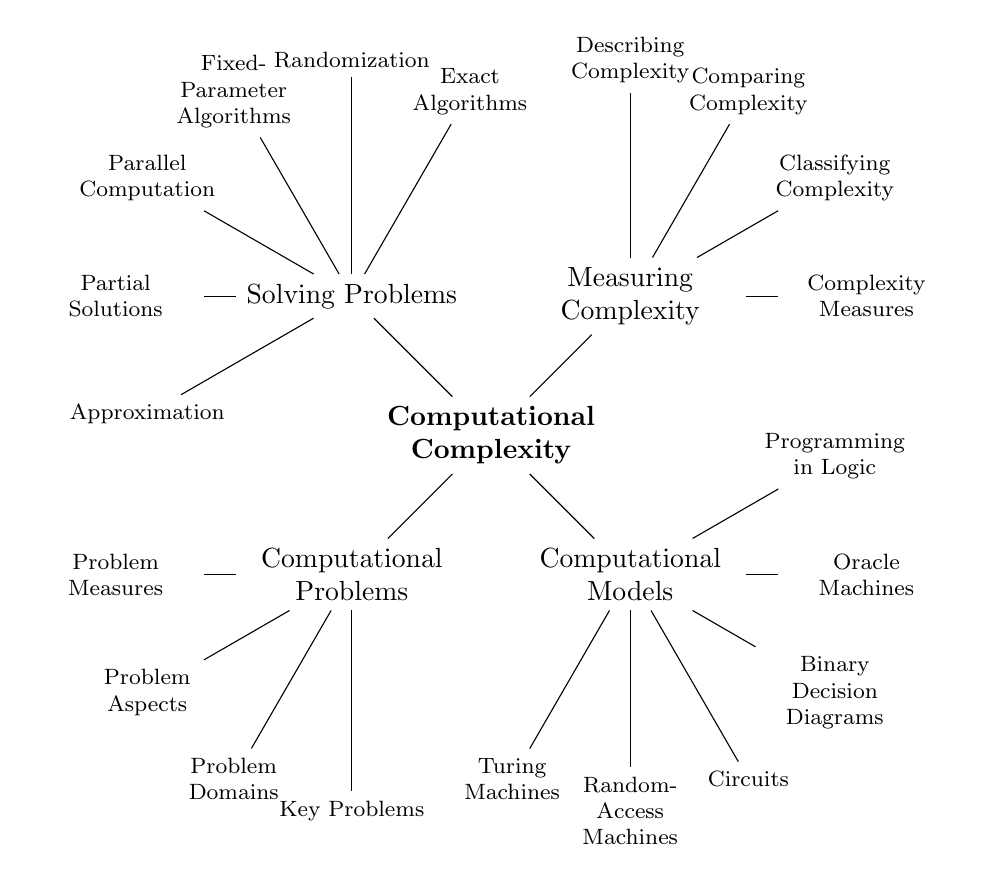
\begin{tikzpicture}[text width=2.7cm, align=flush center,
grow cyclic,
level 1/.style={level distance=2.5cm,sibling angle=90},
level 2/.style={text width=2cm, font=\footnotesize, level distance=3cm,sibling angle=30}]
\node[font=\bfseries] {Computational Complexity} % root
child { 
node {Computational Problems}
child { node {Problem Measures} }
child { node {Problem Aspects} }
child { node {Problem Domains} }
child { node {Key Problems} }
}
child { node {Computational Models}
child { node {Turing Machines} }
child { node {Random-Access Machines} }
child { node {Circuits} }
child { node {Binary Decision Diagrams} }
child { node {Oracle Machines} }
child { node {Programming in Logic} }
}
child { node {Measuring Complexity}
child { node {Complexity Measures} }
child { node {Classifying Complexity} }
child { node {Comparing Complexity} }
child { node {Describing Complexity} }
}
child { node {Solving Problems}
child { node {Exact Algorithms} }
child { node {Randomization} }
child { node {Fixed-Parameter Algorithms} }
child { node {Parallel Computation} }
child { node {Partial Solutions} }
child { node {Approximation} }
};
\end{tikzpicture}
\end{document}